% this intro needs to sound more solemn and deeply curious
Imagine a space that is infinite, featureless, and perfectly symmetric in every direction. A space that has no notion of distance, geometry, or topology, and that is filled with an infinite number of possible states and configurations. A space that is pure potential, waiting to be actualized and shaped by the action of observation.

This is the undifferentiated symmetric morphological space (USMS), the starting point of all existance, for to exist, is merely to differentiate what is and is not. In that sense then, the USMS is everything and it is nothing. <TODO add profound statement that make subtle reference to spiritual and philosophical implications>

In this chapter, we will explore the mathematical and conceptual foundations of the USMS, and we will see how it can be described using the language of Hilbert spaces, symmetry groups, and quantum entanglement.

But why should we start from such an abstract and unfamiliar concept? Why not just take the existence of space and time for granted, as we do in our everyday life? Well, as Einstein taught us with his theory of relativity, space and time are not absolute and unchanging, but are dynamical and intertwined, and they can be bent and stretched by the presence of matter and energy.

And as quantum mechanics has shown us, the fundamental building blocks of reality are not solid and deterministic, but are probabilistic and contextual, and they are subject to the laws of superposition, entanglement, and wave-particle duality. So, if we want to understand the true nature of space and time, and the origin of the laws of physics, we need to go beyond the classical and the intuitive, and we need to embrace the quantum and the abstract.

The USMS is the ultimate quantum and abstract space, the space of all possible spaces, and the foundation of all possible realities. By starting from this space, and by applying the principles of quantum measurement theory and morphic resonance, we will be able to derive the emergence of 3D space, the fundamental quantum fields, and the laws of gravity and cosmology, in a unified and consistent framework.

So, let's put on our mathematical hats and our philosophical shoes, and let's explore the strange and wonderful world of the undifferentiated symmetric morphological space!

\section{Definition and mathematical formulation}
\subsection{Infinite-dimensional Hilbert space representation}
The undifferentiated symmetric morphological space (USMS) is represented as an infinite-dimensional Hilbert space $\mathcal{H}$, which is a complex vector space with an inner product. The elements of $\mathcal{H}$ are the possible states of the USMS, which are represented as vectors $\ket{\psi}$. The inner product between two states $\ket{\psi}$ and $\ket{\phi}$ is denoted as $\braket{\psi|\phi}$, which is a complex number that measures the overlap or similarity between the states.

\begin{tcolorbox}[colback=blue!5!white,colframe=blue!75!black,title=New terms]
\begin{description}
\item[Hilbert space:] A complete inner product space, which generalizes the notion of Euclidean space to infinite dimensions. The state space of a quantum system is represented as a Hilbert space.
\item[Inner product:] A generalization of the dot product that maps two vectors to a scalar quantity and satisfies certain axioms, such as conjugate symmetry and linearity.
\item[Ket notation:] The notation $\ket{\psi}$ represents a vector in a Hilbert space, while $\bra{\psi}$ represents its dual vector. The inner product of two vectors is written as $\braket{\psi|\phi}$.
\end{description}
\end{tcolorbox}

\subsection{Symmetry group and invariance under transformations}
The USMS is invariant under a group of symmetry transformations $G$, which are unitary operators $U(g)$ that act on the states $\ket{\psi}$ as $U(g)\ket{\psi}$. The symmetry group $G$ can be continuous or discrete, and it can include transformations such as rotations, translations, and permutations. The invariance of the USMS under $G$ means that the inner product between any two states is preserved under the action of $U(g)$, i.e., $\braket{\psi|\phi} = \bra{\psi}U(g)^\dagger U(g)\ket{\phi}$.

\begin{tcolorbox}[colback=blue!5!white,colframe=blue!75!black,title=New terms]
\begin{description}
\item[Symmetry group:] A group of transformations that leave a system invariant. The invariance of the USMS under $G$ means that the physical properties of the space are unchanged by the transformations in $G$.
\item[Unitary operator:] A linear operator $U$ that preserves the inner product, i.e., $\braket{U\psi|U\phi} = \braket{\psi|\phi}$ for all states $\ket{\psi}$ and $\ket{\phi}$. Unitary operators represent symmetry transformations in quantum mechanics.
\end{description}
\end{tcolorbox}

\begin{tcolorbox}[colback=green!5!white,colframe=green!75!black,title=Question]
What is the physical meaning of the symmetry group $G$? How does it relate to the observed symmetries of space?
\tcblower
The symmetry group $G$ represents the fundamental symmetries of the USMS, which are the transformations that leave the space invariant at the most basic level. These symmetries are broken by the process of observation and measurement, leading to the emergence of the observed symmetries of space, such as translation, rotation, and Lorentz invariance. The relationship between the symmetries of the USMS and the observed symmetries of space is analogous to the relationship between the symmetries of a high-temperature phase and the broken symmetries of a low-temperature phase in a phase transition.
\end{tcolorbox}

\section{Properties and characteristics}
\subsection{High degree of connectivity and entanglement}
The USMS is characterized by a high degree of connectivity and entanglement between its states, which means that any two states $\ket{\psi}$ and $\ket{\phi}$ are connected by a non-zero inner product $\braket{\psi|\phi}$. The entanglement between the states is measured by the von Neumann entropy $S(\rho) = -\Tr(\rho \log \rho)$, where $\rho$ is the density matrix of the USMS, which is a positive semidefinite operator that describes the statistical properties of the states. The high degree of connectivity and entanglement implies that the USMS has a large amount of information and complexity, which is not accessible to local observations and measurements.

\begin{tcolorbox}[colback=blue!5!white,colframe=blue!75!black,title=New terms]
\begin{description}
\item[Entanglement:] A quantum phenomenon in which the states of two or more systems are correlated in a way that cannot be described by classical probability theory. Entangled states exhibit non-local correlations that are stronger than any classical correlations.
\item[Von Neumann entropy:] A measure of the amount of information or uncertainty in a quantum state, given by the formula $S(\rho) = -\Tr(\rho \log \rho)$, where $\rho$ is the density matrix of the state. The von Neumann entropy is zero for a pure state and positive for a mixed state.
\item[Density matrix:] A matrix that describes the statistical state of a quantum system, given by $\rho = \sum_i p_i \ket{\psi_i}\bra{\psi_i}$, where $p_i$ is the probability of the system being in the state $\ket{\psi_i}$. The density matrix is a generalization of the state vector that can represent both pure and mixed states.
\end{description}
\end{tcolorbox}

\begin{tcolorbox}[colback=green!5!white,colframe=green!75!black,title=Question]
How does the high degree of connectivity and entanglement of the USMS relate to the observed locality and separability of space?
\tcblower
The high degree of connectivity and entanglement of the USMS is in stark contrast to the observed locality and separability of space, where distant regions appear to be independent and non-interacting. This apparent contradiction is resolved by the process of decoherence, which is induced by the interaction between the USMS and the environment (i.e., the measurement apparatus). Decoherence leads to the suppression of the off-diagonal elements of the density matrix, which represent the quantum correlations between the states, and the emergence of classical probabilities and separable states. Thus, the observed locality and separability of space is a consequence of the decoherence of the USMS, which hides the underlying connectivity and entanglement from local observations.
\end{tcolorbox}

\subsection{Absence of classical structures and geometries}
The USMS does not have any classical structures or geometries, such as points, lines, or surfaces, which are emergent properties that arise from the symmetry breaking and morphic resonance processes. The absence of classical structures and geometries means that the USMS is a purely quantum and holographic entity, which cannot be described by the concepts of classical physics and mathematics. The only intrinsic property of the USMS is the inner product between its states, which defines the probability amplitudes and the quantum correlations between them.

\begin{figure}[h]
\centering
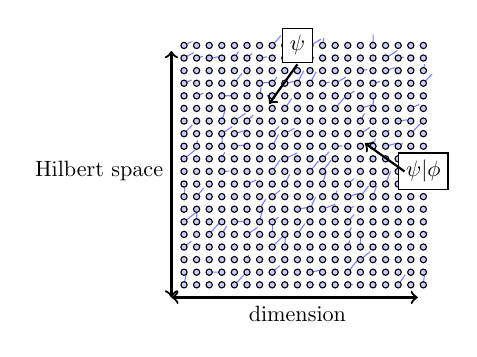
\begin{tikzpicture}[scale=0.8, every node/.style={scale=0.8}]
\foreach \i in {1,...,20}
{
  \foreach \j in {1,...,20}
  {
    \pgfmathparse{rnd} % Calculate a random number
    \pgfmathsetmacro{\prob}{\pgfmathresult} % Store the result in \prob
    \ifdim\prob pt>0.7pt % Compare \prob to 0.7
      \draw[color=blue!50] (\i/5,\j/5) -- (\i/5+rnd/5,\j/5+rnd/5);
    \fi
    \node[draw, circle, fill=blue!20, inner sep=1pt] at (\i/5,\j/5) {};
  }
}
\node[draw, rectangle, fill=white] at (2,4) {$\ket{\psi}$};
\draw[thick, ->, shorten >=2pt] (2,3.7) -- (1.5,3);
\node[draw, rectangle, fill=white] at (4,2) {$\braket{\psi|\phi}$};
\draw[thick, ->, shorten >=2pt] (3.7,2) -- (3,2.5);
\draw[thick, <->, shorten >=2pt] (0,0) -- (0,4) node[midway, left] {Hilbert space};
\draw[thick, <->, shorten >=2pt] (0,0) -- (4,0) node[midway, below] {dimension};
\end{tikzpicture}
\caption{Schematic representation of the undifferentiated symmetric morphological space (USMS) as a highly connected and entangled network of states. The nodes (blue circles) represent the states $\ket{\psi}$ and the edges (blue lines) represent the inner products $\braket{\psi|\phi}$ between them. The absence of classical structures and geometries is indicated by the lack of any regular patterns or symmetries in the network. The labels and arrows explain the meaning of the nodes and edges, and the scale bars indicate the dimensionality of the Hilbert space.}
\label{fig:usms}
\end{figure}